%\documentclass[review]{cvpr}
\documentclass[final]{cvpr}

\usepackage{times}
\usepackage{epsfig}
\usepackage{graphicx}
\usepackage{amsmath}
\usepackage{amssymb}

% Include other packages here, before hyperref.

% If you comment hyperref and then uncomment it, you should delete
% egpaper.aux before re-running latex.  (Or just hit 'q' on the first latex
% run, let it finish, and you should be clear).
\usepackage[pagebackref=true,breaklinks=true,colorlinks,bookmarks=false]{hyperref}


%\def\cvprPaperID{Project Proposal} % *** Enter the CVPR Paper ID here
%\def\confYear{CVPR 2021}
%\setcounter{page}{2} % For final version only


\begin{document}
\title{Deep Learning Project Proposal : Multi-instrument Classification using Partially Labeled Data and Weakly-supervised Learning}

\author{
	Clément Berger\\
	{\tt\small clement.berger@ensta-paris.fr}
% For a paper whose authors are all at the same institution,
% omit the following lines up until the closing ``}''.
% Additional authors and addresses can be added with ``\and'',
% just like the second author.
% To save space, use either the email address or home page, not both
\and Ilyes Er-Rammach\\
{\tt\small ilyes.er-rammach@ensta-paris.fr}

}

\maketitle
\begin{abstract}
	While single-instrument recognition has made tremendous progress, multi-instrument recognition is still considered as a hard task. A part of the difficulty comes from the lack of huge strongly labeled datasets. Recently, a large dataset of polyphonic audio clips called OpenMIC has been released. The drawback of the size of the dataset is that it is only weakly-labeled. Previous works have proposed to use an attention mechanism and a Recurrent Neural Network structure called Bidirectional Long-Short Term Memory (BiLSTM) to train on this dataset. Most works in this field use Log-Mel Spectrograms to treat the audio signal before giving it to the network. Here we explore the use of Continuous Wavelet Transform (CWT) to generate scalograms wich are then given to a Convolutional Neural Network (CNN). Such transformations are supposed to be more efficient in giving a representation of the whole signal. We also test different BiLSTM configurations and try some data augmentation techniques. While we do not improve state of the art, our results are encouraging. With more computational power, pretraining our scalogram-CNN structure as feature extractor using a big dataset like YouTube should be able to achieve great results.
\end{abstract}
\section{Introduction}
\subsection{Motivation}
Multi-instrument recognition is a subfield of Music Information Retrieval (MIR) in which, given a list of instruments and an audio clip, one tries to tell if these instruments figure in the clip or not. Such a task is very useful for music providers to make recommandations based on affinity with some instrument, or to create filters for research and so on. An efficient model could also be used as a basis (like a feature extractor) for other MIR tasks such that source separation, or music transcription.

Such a task requires not only machine learning skills, but also signal processing expertise. Great results have been achieved in single-instrument recognition, see e.g. \cite{mir}. However, polyphonic sounds are the superposition of multiple instruments with different charasteristics and played differently therefore most of these techniques can not be applied for our task.

Another challenge is the difficulty to create datasets. There are roughly two types of datasets of annotated polyphonic sounds. First there are small datasets but very strongly annotated. We can for example cite MusicNet \cite{MusicNet} containing 330 examples. Such datasets face big issues like overfitting. The other type of datasets is huge datasets (at least compared to the previous ones) but only partially labeled. In 2018 has been released a dataset called OpenMIC \cite{MIC} which belongs to the second category. OpenMIC contains 20 000 audio clips of 10 seconds, sampled at 44,1 kHz. However, given an audio clip, we only know if an instrument is in the clip or not but the offset et onset times are not provided. Practically this means that an audio containing 1 second of violin will have the same label as one completely played with a violin. Moreover, there are some missing labels, meaning that given an audio clip, some instrument labels are not provided. 
\subsection{Problem definition}
\subsubsection{Signal processing : different transformations}
\subsubsection{VGGish network}
This section is devoted to briefly present a network created recently for multi-instrument recognition, called VGGish \cite{VGGish_net}. This name simply comes from the fact that it is derived from the classical VGG model \cite{vgg} used for image recognition. Amongst other changes, it has been modified to receive a Log-Mel Spectrogram as entry and the end of the network acts now as a compact embedding layer. A precise definition can be found \href{https://github.com/tensorflow/models/tree/master/research/audioset/vggish}{here}.
\subsubsection{Training using OpenMIC}
In this work we try to train a network on the OpenMIC dataset for multi-instrument recognition. 

The OpenMIC dataset has been labeled with 20 instruments. For each of the 20 000 audio clips and each instruments, we have a binary value indicating if we have a label for this couple (audio, instrument) or not, and if we have so, we also have the probability that the instrument is effectively in the audio clip. In addition of the raw audios and labels, OpenMIC also provides features extracted using the VGGish. More precisely, a Log-Mel Spectrogram is computed for each raw audio, one frame corresponding to 1 second, and then given to the VGGish. After that, a Principal Component Analysis (PCA) is done on the extracted features for each frame. We end up with 10 vectors (one per second) containing 128 features, for each audio clip.
\section{Related work}
\section{Methodology}
\begin{figure}
	\centering
	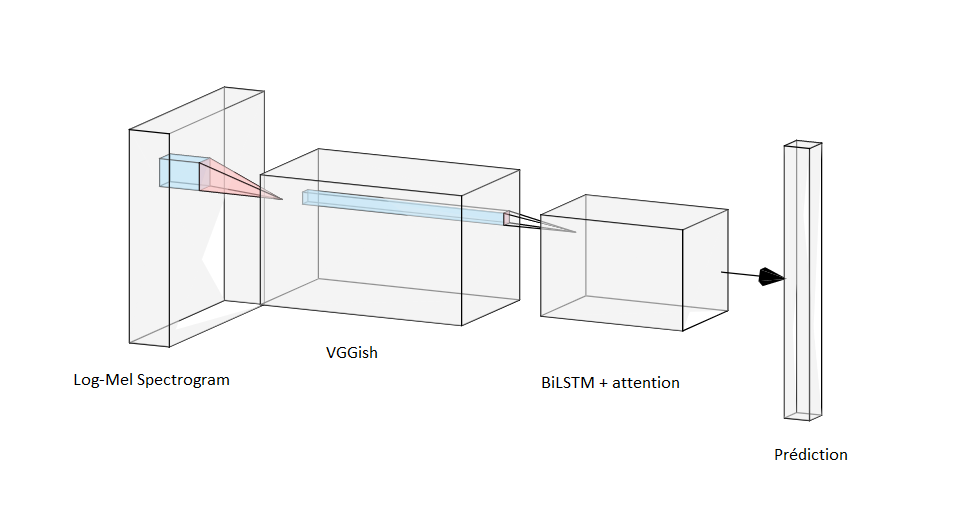
\includegraphics[scale = 0.45]{bilstm.png}
	\caption{Structure using Log-Mel Spectrogram}
	\label{mel}
\end{figure}
\begin{figure*}
	\centering
	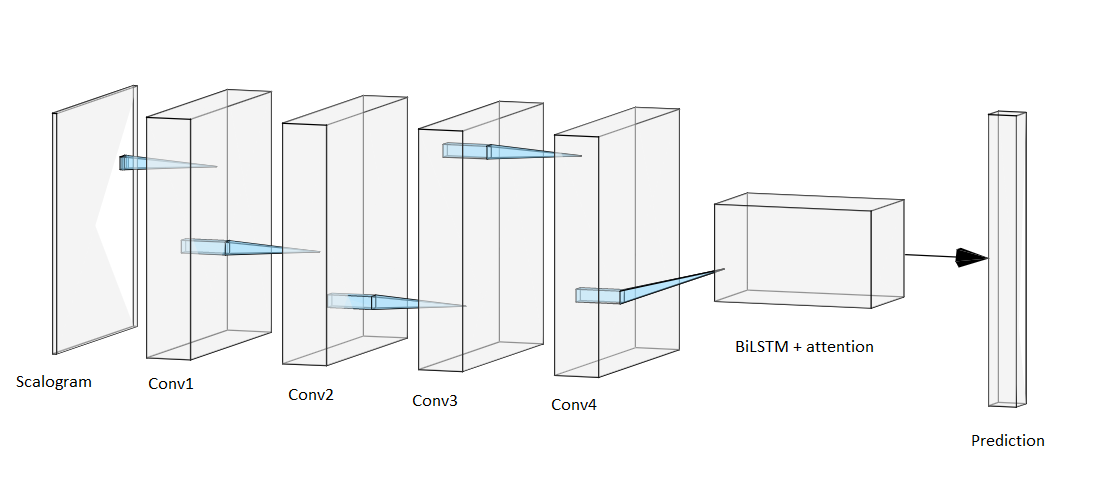
\includegraphics[scale = 0.65]{cnn.png}
	\caption{Convolutional network taking scalograms}
	\label{cnn}
\end{figure*}
\begin{figure}
	\centering
	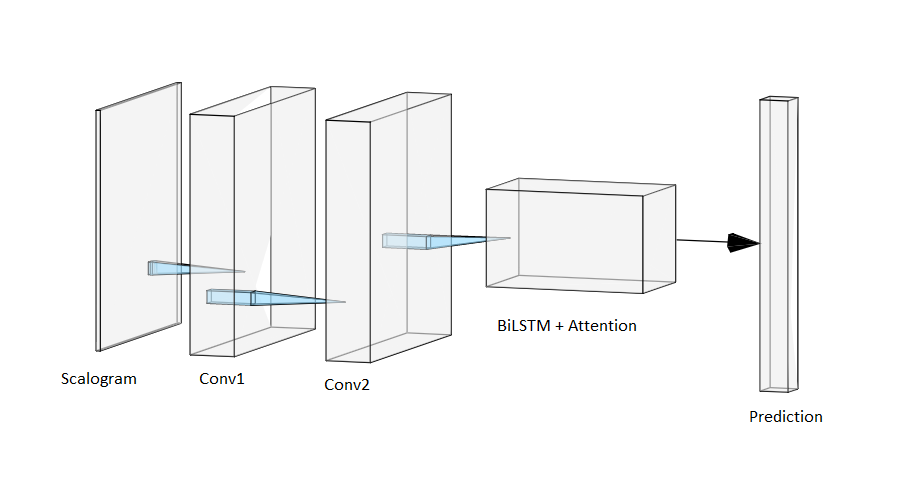
\includegraphics[scale = 0.45]{cnnreduit.png}
	\caption{Convolutional network taking scalograms, reduced structure}
	\label{reduit}
\end{figure}
\section{Motivation and problem definition}
\subsection{Introduction on instrument classification}
Multi-instrument classification consists in, given an audio clip and a list of instruments, telling for each instrument if it is in the audio or not. This task is for example mandatory for users who want to make music research based on instrumental criteria. It can also be useful in the task of genre classification, or for source separation. Recently, researchers have been focusing on machine learning techniques and especially neural networks to solve this problem.

While single-instrument classification has achieved a great level of precision, recognizing instruments within a polyphonic audio clip is still a hard challenge. A big difficulty comes from the fact that a same instrument can be played in very different ways, with for examples different timbres and notes. As a result we get not only that a same instrument can produce very different sounds but also the fact that two different instruments can produce almost the same sound. This difficulty is already the source of a lot of research for single-instrument classification, but adding the superposition of these sounds makes multi-instrument classification a lot harder.

\subsection{About datasets}

Another challenge is the lack of data. Training a neural network requires as many data as possible but there is nothing equivalent to for example ImageNet for instrument recognition. The main datasets are either strongly labeled but with very few samples - see for example MusicNet \cite{MusicNet} with 330 clips - or contain a reasonable amount of samples but with only partial labels. 

In 2018 has been released an open dataset called OpenMIC \cite{MIC} which belongs to the second category. This is the biggest open dataset for multi-instrument classification, with 20 000 (10-second) audio clips. The drawback of this huge number of clips (compared to the other existing datasets) is the fact that the dataset is only weakly-labeled, which means that given an audio clip, we only know the presence or absence of an instrument, without any clue on the onset or offset times. Moreover, given an audio clip, not all instruments are labeled, which means that there are instruments for which we don't know if they are in the audio or not. These constraints make the training of a network a lot harder, however the size of the dataset makes it interesting to study.

\subsection{Our problem}

Given an audio clip and a list of instruments, we aim to determine, for each instrument, if it is played during the audio or not. Our goal is to train a neural network to achieve this task, using the OpenMIC dataset. The underlying goal of using this dataset is to try to find out how to exploit weakly and partially labeled data. 

Recently Amir Kenarsari-Anhari \cite{squelette_progr} got great results training a network on OpenMIC for this purpose. His paper will be the basis of our work, in the sense that we will try to improve his algorithm, as we will discuss in the next section.
\section{Methodology}
\subsection{Squeletton of the algorithm}
Let's briefly describe the algorithm of \cite{squelette_progr}. Given an audio clip, we compute its log mel-spectrogram, which consists in a transformation of the signal (in the same sense than a Fourier transform). This is then given to a Convolutional Neural Network (CNN). Its structure is close to the one of the VGG network used in image recognition, reason why it will be referred as the VGGish layer \cite{VGGish_net}. The next step is to use an attention layer which consists in learning signifiant segments in the clip, see \cite{attention}. This ends with a classification layer.

Our work will follow the structure of this model. Our goal will be to modify some of these blocks to try to improve the performances of the algorithm.
\subsection{Changing the feature learning}
As we discussed, multi-instrument classification and single-instrument classification are pretty different fields. However they both have to deal with the pre processing of the signal. This summer Dutta \etal \cite{features_descr} experimented a scalogram different from the mel-scalogram to train a network on single-instrument classification. The idea of their technique is to use features computed on the whole signal while other methods subdivise the signal before processing each part. As they achieved greater results than previous works, our idea would be to try to use this scalogram for our model to get maybe more representative features which would hopefully result in a better training. 

Another modification indirectly suggested by this paper would be to even change the VGGish layer and use the one of Dutta \etal. This would allow us to try different CNN for this part of the algorithm.

We also note that Dutta \etal trained only on 14 instruments (compared to 20 in OpenMIC). Experimenting it on our algortihm will so be a double test, trying not only a different task but also different instruments.
\subsection{Data augmentation}
As Amir Kenarsari-Anhari suggested at the end of his paper, another direction of research to improve his model is to experiment more data augmentation. Our primary goal will be to experiment on changing the feature learning process, but if possible we plan to try to add different data augmentation techniques, as it is a natural way to try to deal with the small size of the dataset. 

A starting point may be a paper from Schlüter and Grill \cite{data_aug} using data augmentation for singing voice detection. Even if voice detection is quite different from instrument classification, this paper presents data augmentation techniques which are a bit more general than just voice detection. Moeover we can also try to take some of the techniques specific to voice detection and to adapt them to our problem, potentially leading to new techniques.
\section{Evaluation}
We will first try to implement the changes discussed in 2.2., namely changing the scalogram and the VGGish layer. If it's possible, we will then explore some data augmentation techniques. We will experiment different combinations of our changes and compare them at first to the results of \cite{squelette_progr} to see if we are able to achieve a better performance. We will also make comparisons between them to try to find out the most effective one(s) and try to deduce some interpretation of why some are better than the others. As our purpose is to improve the algorithm of \cite{squelette_progr}, it will constitute our benchmark, meaning that we will focus on comparing our best results with theirs. 

We precise that the performances of an algorithm are not measured in terms of the usual accuracy in the field of instrument classification. Indeed, as some instruments are easier than others to recognize, a difference of accuracy doesn't perfectly reflect an improvement in the classification of hard instruments. Therefore we will use the F1 score which is a metric created specificaly for this purpose. Details can be found in \cite{metric}. In order to produce a meaningful comparison, we will more precisely use the parameters that are described in \cite{squelette_progr}.
{\small
	\bibliographystyle{ieee_fullname}
	\bibliography{report}
}
\end{document}